\documentclass{article}

\usepackage{graphicx}
\usepackage{tikz}
\usepackage{tikzsymbols}
\usetikzlibrary{calc,patterns,shapes.geometric}
\pagestyle{empty}
\usepackage[margin=0pt]{geometry}
\geometry{papersize={14in,12in}}

\def\centerarc[#1](#2)(#3:#4:#5){\draw[#1] ($(#2)+({#5*cos(#3)},{#5*sin(#3)})$) arc (#3:#4:#5);}

\begin{document}
	\begin{figure}
		\centering
		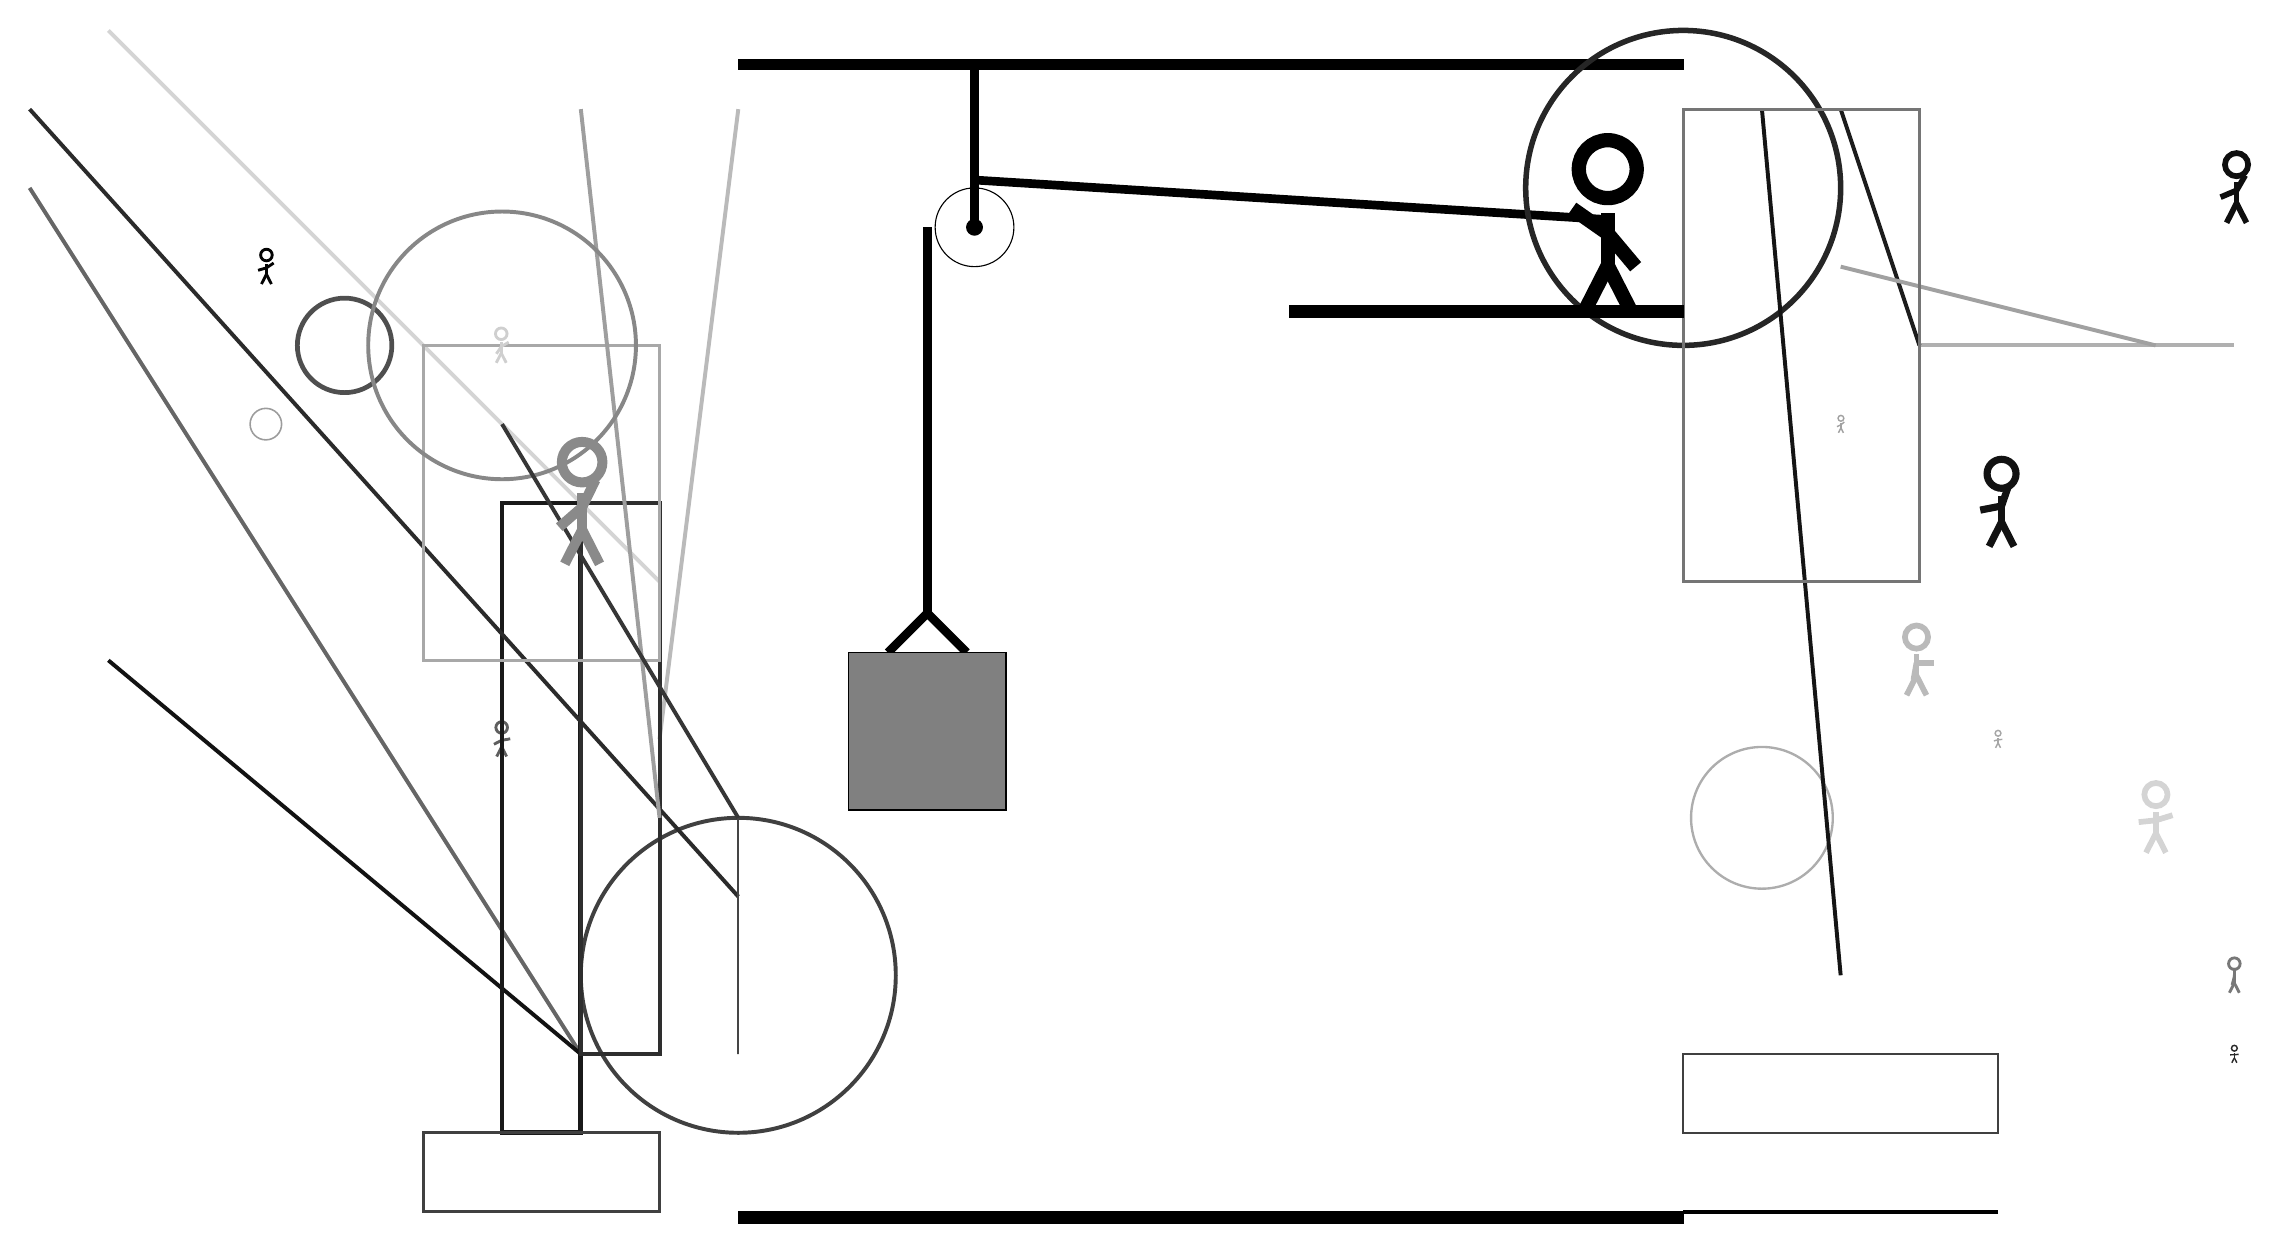
\begin{tikzpicture}
			%%%%% START %%%%%
			
			\draw[fill=black] (-2, 11.5) rectangle (10, 11.625);
			
			\draw (1, 9.5) circle (0.5);
			\draw[fill=black] (1, 9.5) circle (0.1);
			\draw[line width=1.1mm] (1, 11.5) -- (1, 9.5);
			
			\draw[line width=1.1mm](-0.1, 4.1) --  (0.4, 4.6) -- (0.9, 4.1);
			\draw[fill=black!50] (-0.6, 4.1) rectangle (1.4, 2.1);
			
			\draw[line width=1.1mm](0.4, 9.5) -- (0.4, 4.6);
			\centerarc[line width=1.1mm](1, 9.5)(90:180:0.6)
			\draw[line width=1.1mm](1, 10.1) -- (9, 9.6);
			
			\draw[line width=0.5mm, color=black!31](13, 8) -- (17, 8);
			
			\draw[line width=0.5mm, color=black!60](-4, -1) -- (-11, 10);
			\draw [line width=0.6mm, color=black!69](-7, 8) circle (0.6);
			\node[line width=0.4mm, color=black!99] at (-8, 9) {\Strichmaxerl[2][16][34]};
			\draw[line width=0.5mm, color=black!17](-3, 5) -- (-10, 12);
			\node[line width=0.7mm, color=black!63] at (-5, 3) {\Strichmaxerl[2][27][10]};
			\node[line width=0.6mm, color=black!93] at (14, 6) {\Strichmaxerl[5][11][71]};
			\draw[line width=0.5mm, color=black!27](-2, 11) -- (-3, 3);
			\draw [line width=0.2mm, color=black!39](-8, 7) circle (0.2);
			\node[line width=0.7mm, color=black!27] at (13, 4) {\Strichmaxerl[4][80][0]};
			\draw[line width=0.5mm, color=black!89](12, 11) -- (13, 8);
			
			\draw[line width=0.5mm, color=black!93](-4, -1) -- (-10, 4);
			\draw [line width=0.5mm, color=black!75](-2, 0) circle (2.0);
			
			\draw[line width=0.6mm, color=black!90] (-4, 6) rectangle (-5, -2);
			\draw [line width=0.7mm, color=black!85](10, 10) circle (2.0);
			\draw[line width=0.5mm, color=black!82] (-4, 6) rectangle (-3, -1);
			
			\node[line width=0.4mm, color=black!37] at (12, 7) {\Strichmaxerl[1][26][39]};
			
			\draw[line width=0.5mm, color=black!83](-2, 1) -- (-11, 11);
			\draw[line width=0.3mm, color=black!34] (-3, 4) rectangle (-6, 8);
			\draw [line width=0.3mm, color=black!32](11, 2) circle (0.9);
			\node[line width=0.3mm, color=black!94] at (17, 10) {\Strichmaxerl[4][23][60]};
			
			\node[line width=0.3mm, color=black!17] at (16, 2) {\Strichmaxerl[4][6][17]};
			\draw[line width=0.3mm, color=black!75] (10, -2) rectangle (14, -1);
			\draw[line width=0.3mm, color=black!73] (-2, 2) rectangle (-2, -1);
			\draw[line width=0.5mm, color=black!38](-4, 11) -- (-3, 2);
			\node[line width=0.2mm, color=black!84] at (17, -1) {\Strichmaxerl[1][2][4]};
			\draw[line width=0.5mm, color=black!92](12, 0) -- (11, 11);
			\draw[line width=0.5mm, color=black!37](12, 9) -- (16, 8);
			
			\draw[line width=0.4mm, color=black!54] (10, 11) rectangle (13, 5);
			
			\draw [line width=0.5mm, color=black!47](-5, 8) circle (1.7);
			\draw[line width=0.5mm, color=black!100](14, -3) -- (10, -3);
			
			\node[line width=0.5mm, color=black!35] at (14, 3) {\Strichmaxerl[1][17][4]};
			\draw[line width=0.5mm, color=black!79](-2, 2) -- (-5, 7);
			\draw[line width=0.4mm, color=black!75] (-3, -2) rectangle (-6, -3);
			
			\node[line width=0.4mm, color=black!53] at (17, 0) {\Strichmaxerl[2][75][88]};
			\node[line width=0.4mm, color=black!19] at (-5, 8) {\Strichmaxerl[2][56][31]};
			\node[line width=0.6mm, color=black!46] at (-4, 6) {\Strichmaxerl[7][41][64]};
			
			
			\node at (9, 9.5) {\Strichmaxerl[10][-35][-50]};
			\draw[fill=black] (5, 8.5) rectangle (10, 8.35);
			
			\draw[fill=black] (-2, -3) rectangle (10, -3.15);
			
			%%%%% END %%%%%
		\end{tikzpicture}
	\end{figure}	
\end{document}